\documentclass{article}
\usepackage[utf8]{inputenc}
\usepackage{geometry}
\usepackage{graphicx}
\usepackage{pgfplots}
\usepackage{amsmath}
\usepackage{amssymb}
\usepackage{amsfonts}
\usepackage{mdframed}
\usepackage{amsthm}
\usepackage{tikz}
\usepackage{multicol}
\usepackage{cancel}
\usepackage{hyperref}

\geometry{a4paper, left=2cm, right=2cm, top=1cm, bottom=2cm}

\pgfplotsset{compat=1.18}
\begin{document}

\begin{minipage}{0.7\textwidth}
    \small \textbf{LABORATORIO DE MECÁNICA VECTORIAL}  \\
    \small {Facultad de Ciencias, Universidad Nacional Autónoma de México} \\
    \small {Profesor: Radamés Ricardo Reynoso Manríquez} \\
    \small {Ayudante: Ana Laura Córdova Lara}\\
    \small {Fecha de entrega: 05 de Mayo de 2024} \\
    \small {Integrantes del equipo: López González Andrés \\
    \small Mendoza Lara José Alfredo, Vallejo Mendoza José Daniel} \\
    \small {Informe Número IX}
\end{minipage}
\hfill
\begin{minipage}{0.12\textwidth}
    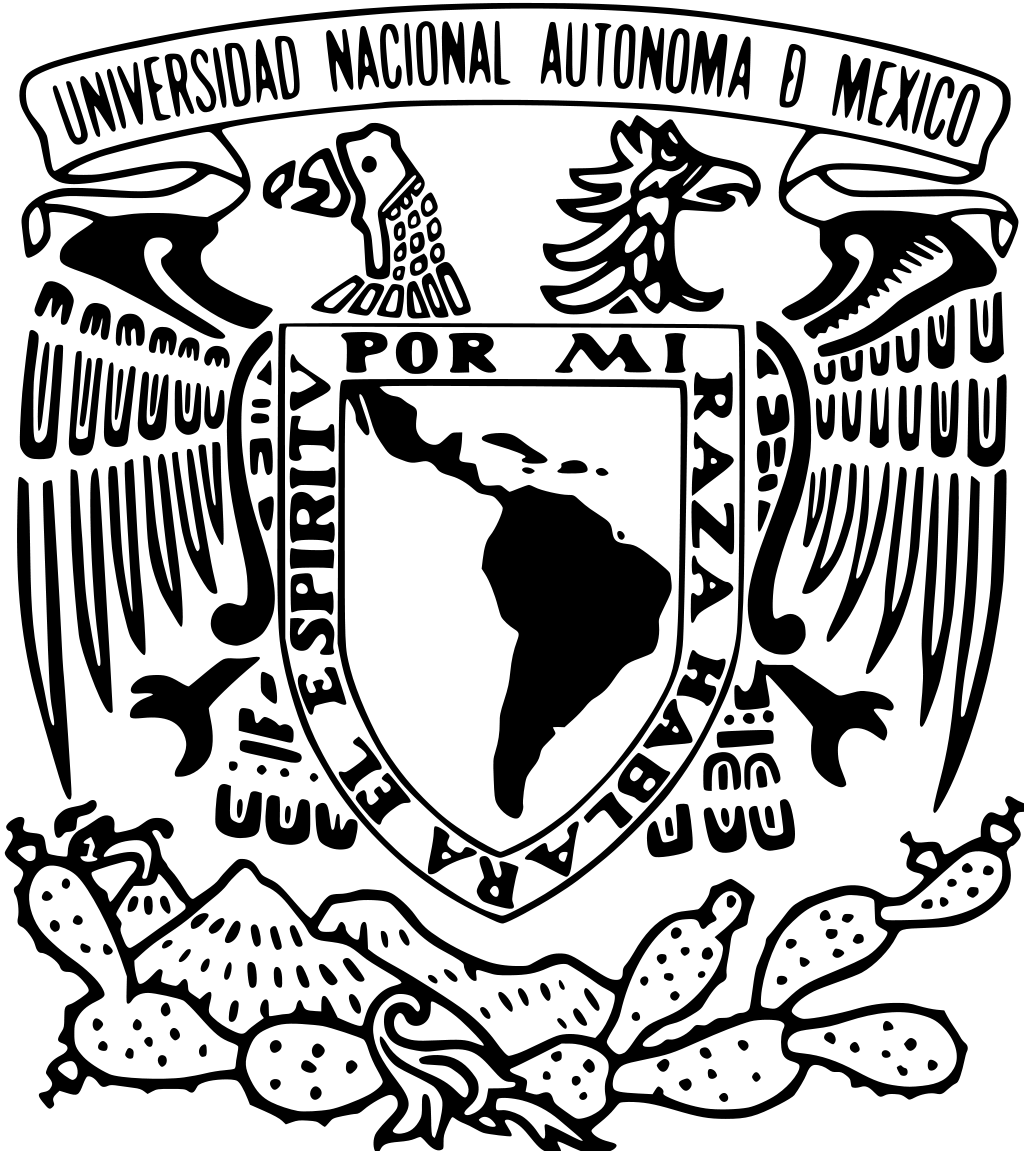
\includegraphics[width=\linewidth]{logo_universidad}
\end{minipage}
\section{Movimiento rectilíneo con fuerza constante.}

\subsection{Abstract:}
Las fuerzas están presentes a lo largo de todo el universo, son las que mantienen a los átomos unidos; son las que mantienen los enlaces entre las moléculas de los compuestos que nos rodean. Más específicamente, a nivel macroscópico, las fuerzas se vuelven más aparentes junto con sus consecuencias. En este documento se exponen los datos obtenidos y los hechos que los relacionan, de manera que podamos llegar experimentalmente a los hechos que nos son expuestos tanto por la observación del mundo físico, como por la intuición matemática detrás del mismo.\\

\subsection{Introducción:}
Describir a las fuerzas físicamente puede ser un poco más intrincado de lo que verdaderamente es, pues una larga vida de estar acostumbrados a usar la etiqueta de fuerza para describir sucesos que experimentamos en el día a día nos ha mal acostumbrado. Empleamos la palabra para describir: empujes, jalones, intensidad entre otros; y, si bien nuestra intuición en primera instancia no está tan lejos de la verdad, nuestro deber como proscritos de la ciencia es buscar una definición a partir de lo que les es común a todas estas vivencias que la experiencia empírica nos ha dejado.\\
Así pues, la física describe a la fuerza como una interacción entre cuerpos y, redundantemente, es este concepto el que le da su razón de ser a la física, pues es la rama de la ciencia que estudia las interacciones entre la materia. Aunque es verdad que su definición se vuelve progresivamente más difusa mientras más nos adentramos en las ramas que encapsula la física, lo anterior es completamente verdadero para la física newtoniana.
\subsection{Marco teórico:}
La física falla en describir al universo de la manera más fiel posible, pues si tomamos en cuenta todas las variables involucradas, hasta el más simple de los fenómenos se puede tornar en una complejidad que resulta contraproducente a la tarea de entender mejor las leyes que en conjunto forman y rigen la naturaleza.\\
El modelo simplificado para un cuerpo que se mueve y cambia constantemente de velocidad bajo la acción de una fuerza en mecánica clásica consiste en tomar al cuerpo como una partícula puntual; suponer, para facilitar los cálculos, que el sistema de referencia sobre el que está montado es inercial. Lo anterior nos ayuda a simplificar el análisis de las fuerzas que actúan sobre el cuerpo para que el fenómeno de superposición de fuerzas sea aplicable y, de esta manera, podamos usar la segunda ley de newton para calcular la aceleración, la masa o la fuerza neta (dependiendo de los datos de los que dispongamos). Lo anterior nos es posible por el enunciado de la primera ley de Newton; sabemos que conceptos son aplicables al fenómeno por lo que esta enuncia.\\
La fuerza externa provoca el cambio en la velocidad del cuerpo, es decir, en su rapidez o en su dirección; la aceleración producida debido a esta tiene la misma dirección que tiene la fuerza neta (la sumatoria de fuerzas que actúan sobre el cuerpo) lo que indica que la fuerza es una magnitud de carácter vectorial.\\
\begin{equation}
    \sum \Vec{F} = m\Vec{a}
\end{equation}

Está relación nos dice que, si la fuerza neta que experimenta el cuerpo es constante, su aceleración también lo será, tanto en magnitud como en dirección. Si la condición anterior se cumple, entonces la aceleración media es igual a la aceleración instantánea del cuerpo.\\
\begin{equation}
    \Bar{}{a_{ins}} = \frac{d^{2}x}{dt^{2}} = \frac{\Delta \Bar{v}}{\Delta t} = \frac{\Sigma\Bar{F}}{m} = \Bar{a_{med}}
\end{equation}

Para saber cuales son las fuerzas que está experimentando un cuerpo hay que preguntarse qué cuerpos son los que interactúan sobre el cuerpo y cuál es su naturaleza: si es una fuerza de contacto o por el contrario es una fuerza de alcance como lo es la fuerza de gravedad en la tierra. Una vez identificadas todas las fuerzas, auxiliados de un diagrama de cuerpo libre, podemos calcular el valor de la fuerza neta mediante la sumatoria vectorial de las componentes.\\
\begin{figure}
    \centering
    
\includegraphics[width=0.5\linewidth]{Diagram.png}
    \caption{Diagrama de cuerpo libre para un cuerpo sobre un plano horizontal e inclinado.}
    \label{fig:enter-label}
\end{figure}

En el caso de un sistema compuesto por dos masas unidas por una cuerda/hilo que pasa por una polea, si la masa de cuerda es despreciable porque las masas de los otros cuerpos son muy grandes en comparación a esta, la tensión en la cuerda es la misma en todos los puntos pues\\
\begin{equation}
    \Sigma \Bar{F_{cuerda}} = T_{1} - T_{2} = m\Bar{a} = 0
\end{equation}
 
\subsection{Objetivo:}
Dada las masas de los cuerpos y las fuerzas aplicadas sobre ellos, evaluar y registrar el movimiento de los cuerpos empleando una metodología experimental en un ambiente controlado.\\
Calcular la aceleración a partir de un desplazamiento medido y cotejar los datos con las fórmulas matemáticas suministradas por la teoría; en caso de que las mediciones no sean congruentes, reportar los hechos que impidieron la culminación exitosa del experimento a través del análisis de los datos y el recuento de los pasos seguidos a lo largo del proceso.\\

\subsection{Materiales y métodos:}
\begin{itemize}
    \item Carro de baja fricción (PASCO) 
    \item Riel de aire (o riel de baja fricción)
    \item Dinamómetro
    \item Pesas
    \item Ligas 
    \item Balanza
    \item Plastilina
    \item Hilo de cáñamo.
    \item Cronómetro
    \item Flexómetro
    \item Compresora
    \item Polea de baja fricción
\end{itemize}\\\\

Para la primera parte, se instaló el riel de baja fricción y se niveló; Se pegó a un costado con cinta adhesiva el flexómetro para medir el desplazamiento; se instaló las ligas a los extremos del riel para evitar que el deslizador no se estrellara estrepitosamente contra el riel y se dañara el equipo; después se conectó a la compresora de aire. \\
Una vez instalado el equipo, se pesó el deslizador con la balanza para después agregar plastilina cuidadosamente para que pesara 1kg  y se facilitaran los cálculos; se identificó el origen del eje de coordenadas, y seguidamente, uno de nuestros compañeros llevó a cabo la tarea de aplicarle una fuerza constante al deslizador, fuerza que se midió conectando un dinamómetro en el extremo del mismo. Se midió con un cronómetro el tiempo que este tardaba en recorrer cierta distancia mientras estaba siendo afectado por la fuerza, y también se midió la distancia que recorría en un tiempo cuando la fuerza dejaba de ser aplicada.\\

En la segunda parte del experimento, se conectó un hilo de masa despreciable al extremo del deslizador, se le hizo pasar por una polea de baja fricción y, del extremo opuesto, se le añadió una masa conocida de plastilina la cual se dejó constante para todas las mediciones. La masa que varió fue la del deslizador, pues facilitaba el proceso a la hora de variar las masas.. Se soltó el sistema deslizador-masa del reposo y se midió con el cronómetro el tiempo que tardaba en recorrer un desplazamiento determinado.\\

\subsection{Resultados:}
En la primera parte del experimento fue sumamente complicado hacer las mediciones de forma adecuada, por razones como la dificultad de mantener constante la fuerza en el dinamómetro y el hecho de que el riel de baja fricción no tiene una longitud suficiente para medir un recorrido amplio.\\

En la segunda parte, se realizaron 10 mediciones con cada una de las 10 diferentes masas en el carro de baja fricción, y los resultados obtenidos fueron promediados y registrados en la siguiente tabla\\

\begin{center}
\begin{table}[h]
\begin{tabular}{|c|c|}
\hline
\textbf{Masa del Carro} & \textbf{Desplazamiento horizontal en 1 segundo} \\ \hline
1 kg                    & 50.021 cm                                       \\ \hline
0.5 kg                  & 99.605cm                                        \\ \hline
0.6 kg                  & 83.042 cm                                       \\ \hline
0.7 kg                  & 71.146 cm                                       \\ \hline
1.3 kg                  & 38.309 cm                                       \\ \hline
1.45 kg                 & 34.341 cm                                       \\ \hline
1.6 kg                  & 32.022 cm                                       \\ \hline
1.8 kg                  & 26.995 cm                                       \\ \hline
1.9 kg                  & 26.331 cm                                       \\ \hline
2.0 kg                  & 24.864 cm                                       \\ \hline
\end{tabular}
\end{table}
\end{center}

Tabla I. Mediciones registradas de distancia recorrida, con masa variable y fuerza constante.\\\\

Estos datos al ser representados en un plano masa vs desplazamiento y aplicar las ecuaciones de la regresión lineal se observan de la siguiente forma:\\

\begin{figure}[h]
    \centering
    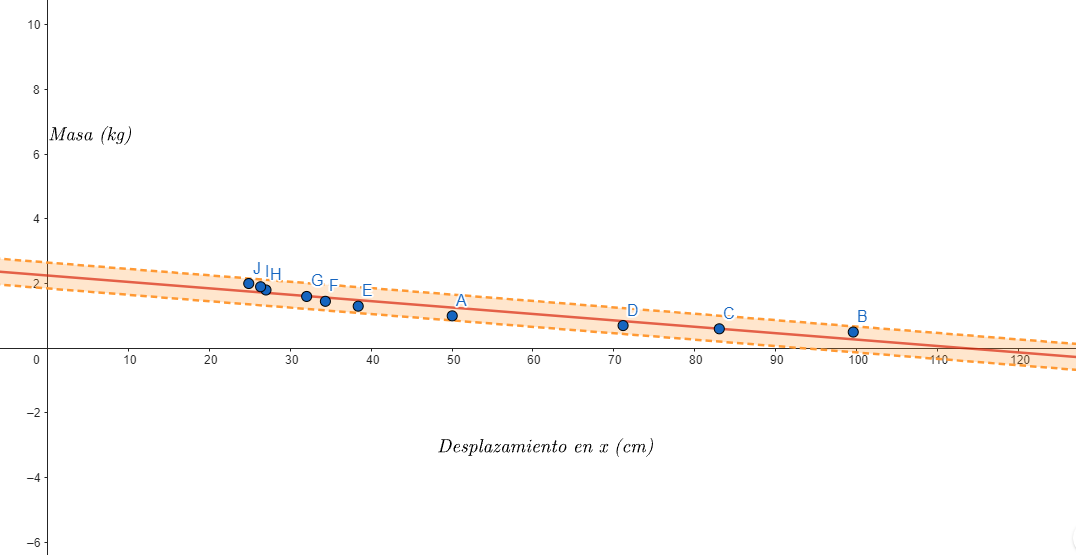
\includegraphics[width=0.75\linewidth]{Regresion.png}
    \caption{Regresión lineal del desplazamiento en función de la masa.}
    \label{fig:enter-label}
\end{figure}\\

\subsection{Discusión de resultados:}
En la primera parte del experimento nos fue imposible registrar con exactitud los datos debido a factores de diversa naturaleza como lo son por ejemplo, la funcionalidad y características de los materiales y equipo empleados.\\
El primer obstáculo al que nos enfrentamos, fue que era extremadamente complicado aplicarle una fuerza constante al deslizador mientras se desplazaba, y a su vez, la longitud limitada del riel nos daba muy poco margen de error; a pesar de que se emplearon dinamómetros de diferente sensibilidad, nuestros esfuerzos se vieron frustrados con cada intento por lo anteriormente mencionado.\\

En la segunda parte, las mediciones se facilitaron, pues la fuerza constante que se aplicaba dependía completamente de la masa que tenía el deslizador, y nuestros resultados fueron congruentes con lo que nos dice la teoría. Conocidas las masa del deslizador y el contrapeso, el desplazamiento del deslizador en un tiempo determinado, y el hecho de que se soltaba al sistema desde el reposo, se pudo utilizar la ecuación proporcionada por el diagrama del cuerpo libre sobre el deslizador.\\
\begin{equation}
    \Sigma F_{x} = T = m\Bar{a} = \frac{m}{\Delta t^{2}} \cdot (2\Delta x)
\end{equation}

En el que se supone que la fricción entre el deslizador y la superficie es despreciable. \\
Una vez calculada la tensión que sufre el hilo, se analiza el diagrama de cuerpo libre del contrapeso que es a lo largo del eje y.\\
\begin{equation}
    \Sigma \Bar{F_{y}} = W - T = m\Bar{a}
\end{equation}

Nótese que el peso no es negativo a pesar de que se dirige hacia abajo; esto es porque se tomó la orientación de las fuerzas en términos de la dirección del movimiento del sistema. En este caso, la tensión es la que va en sentido contrario al movimiento del contrapeso.
Con esta ecuación, se despeja la masa, se divide la fuerza neta a lo largo del eje Y entre la aceleración del sistema, y, de esta manera, cotejamos que nuestros datos sean congruentes, pues se midió previamente la masa del contrapeso.\\

\subsection{Conclusiones:}
A pesar de las dificultades sufridas en la primera parte del experimento, se pudo, en la segunda parte, inferir correctamente en la relación que existe entre la fuerza que experimenta un cuerpo y su movimiento. Además de que se logró modelar con éxito un sistema compuesto por dos cuerpos y una tensión intermediaria aplicando una metodología rigurosa y experimental. 
Se pudo apreciar lo esperado: la tasa de cambio constante de la velocidad del deslizador en función del tiempo para un desplazamiento dado. Entre más disminuye la masa del deslizador, mayor es la aceleración que sufre, pues la aceleración es inversamente proporcional a la masa del cuerpo en cuestión.

\subsection{Referencias:}
\begin{itemize}
    \item Smith, J. (2019). Understanding Motion: An Introduction to Uniform Rectilinear Motion. New York, NY: Publisher.
    \item García, M., \& López, A. (2020). Análisis del Movimiento Rectilíneo Uniforme en la Educación Secundaria. Revista de Educación Científica, 15(2), 45-58.
    \item Johnson, R. (2018). Physics of Motion: Exploring Uniform Rectilinear Motion. Journal of Physics Education, 25(3), 112-125. DOI: 10.1080/12345678.2018.1234567
    \item Halliday, D., Resnick, R., \& Walker, J. (2013). Fundamentals of Physics (10th ed.). John Wiley \& Sons.
\end{itemize}

\subsection{Apéndice:}\\
\textit{Además de la amplia lista de ecuaciones para análisis de incertidumbres y regresión lineal se ha empleado lo siguiente.}
\begin{equation*}
    \Sigma \Bar{F} = m\Bar{a}
\end{equation*}
\begin{equation*}
    \Bar{}{a_{ins}} = \frac{d^{2}x}{dt^{2}} = \frac{\Delta \Bar{v}}{\Delta t} = \frac{\Sigma\Bar{F}}{m} = \Bar{a_{med}}
\end{equation*}
\begin{equation*}
    \Sigma \Bar{F_{cuerda}} = T_{1} - T_{2} = m\Bar{a} = 0
\end{equation*}
\[T_{1} = T_{2}\]
% $m = 0 y T_{1} - T_{2} = 0; T_{1} = T_{2} $
\begin{equation*}
    \Sigma F_{x} = T = m\Bar{a} = \frac{m}{\Delta t^{2}} \cdot (2\Delta x)
\end{equation*}
\begin{equation*}
    \Sigma \Bar{F_{y}} = W - T = m\Bar{a}
\end{equation*}


\end{document}